\FloatBarrier
\section{Performance of the newer Algorithms Compared to Classical Sorting Networks} 
\label{sec:Performance}

The first set of experiments measure the performance of the newly developed algorithms Randomized Shellsort and Annealing Sort, respectively of~\citeA{RandShellSort} and~\citeA{AnnealingSort} and compare them to that of the classical sorting networks Bitonic Sort and Odd-Even Mergesort of~\citeA{SNApplications}.

Input sizes are chosen as a power of 2, in order to allow Bitonic Sort and Odd-Even Mergesort to exploit known input sizes for compiler optimization.

The algorithms do not use SIMD, CUDA or OpenMP, as these techniques are the subject of separate experiments.
The use of a fixed sorting network for low sizes of Randomized Shellsort is not used, as it pollutes the number of comparisons while providing only a small performance gain.
Annealing Sort is run with the parameters $(g_{scale}, h, q, c) = (0, 1, 1, 10)$. The meaning and value of these parameters is further discussed in Section~\ref{sec:AnnealingSortImplementation} and~\ref{sec:AnnealingExperiments}.
Odd-Even Mergesort uses a buffer to separate odd and even elements, as the performance degradation of not doing so is massive, and further discussed in Section~\ref{sec:OEMergesortExperiment}. Additionally, Odd-Even Mergesort will use the strategy of performing two recursive layers per pass through the data. 

Pratt's Shellsort and Shaker Sort will not be shown in this section, but are instead evaluated in Section~\ref{sec:ShellsortExperiments}.

\texttt{std::sort} is included as a reference implementation of sorting.

\subsection{Running Time and Comparisons}

First and foremost, we must ensure that the algorithms conform to the expected complexities of $O(n \log n)$ and $O(n \log^2 n)$. If they do not do this, especially in the case of comparisons, then something hints at an erroneous implementation, or some other unexpected factor affecting performance.

First, let us consider comparisons. Figure~\ref{fig:Performance:comparisons} shows the number of comparisons performed for each algorithm.  Keep in mind that the x-axis is logarithmic and the y-axis is divided by $n \log n$, which makes $O(n \log n)$ approach a flat line and $O(n \log^2 n)$ approach a straight line.

It is clear that that Randomized Shellsort performs a number of comparisons that is $O(n \log n)$, and the constant factor is slightly below $5$, which appears consistent with theory.

Bitonic Sort and Odd-Even Merge sort both perform $O(n \log^2 n)$ comparisons, as seen by the linear growth in y-axis from exponential growth in x-axis, and, as expected, we see Odd-Even Mergesort perform slightly fewer comparisons than Bitonic Sort. Note that the despite being $O(n \log^2 n)$, the amount of comparisons performed by these two algorithms is actually not overly large.

Annealing Sort appears periodic in the number of comparisons, but it also appears to be constrained between 10 and 12. This periodic behaviour can be attributed to integer rounding of the $r$ parameter of the annealing sequence, as this is computed as $\frac{\log n}{\log \log n}$, in floating point arithmetic, but must by necessity of the annealing sequence be reduced to an integer.\footnote{
{
\begin{adjustwidth}{-.5in}{-.5in}
\centering
\begin{tabular}{|c|c|c|c|c|c|c|c|c|c|c|c|c|c|c|c|}
\hiderowcolors
\hline
$n$                          & $2^{10}$ & $2^{11}$ & $2^{12}$ & $2^{13}$ & $2^{14}$ & $2^{15}$ & $\mathbf{2^{16}}$ & $2^{17}$ & $2^{18}$ & $2^{19}$ & $2^{20}$ & $2^{21}$ & $2^{22}$ & $\mathbf{2^{23}}$ & $2^{24}$ \\ \hline
$\frac{\log n}{\log \log n}$ & 3.01   & 3.18   & 3.35   & 3.51   & 3.68   & 3.84   & \textbf{4.00}   & 4.16   & 4.32   & 4.47   & 4.63   & 4.78   & 4.93   & \textbf{5.08} & 5.23   \\ \hline
\end{tabular}
\end{adjustwidth}
}
}

\begin{figure}
\center
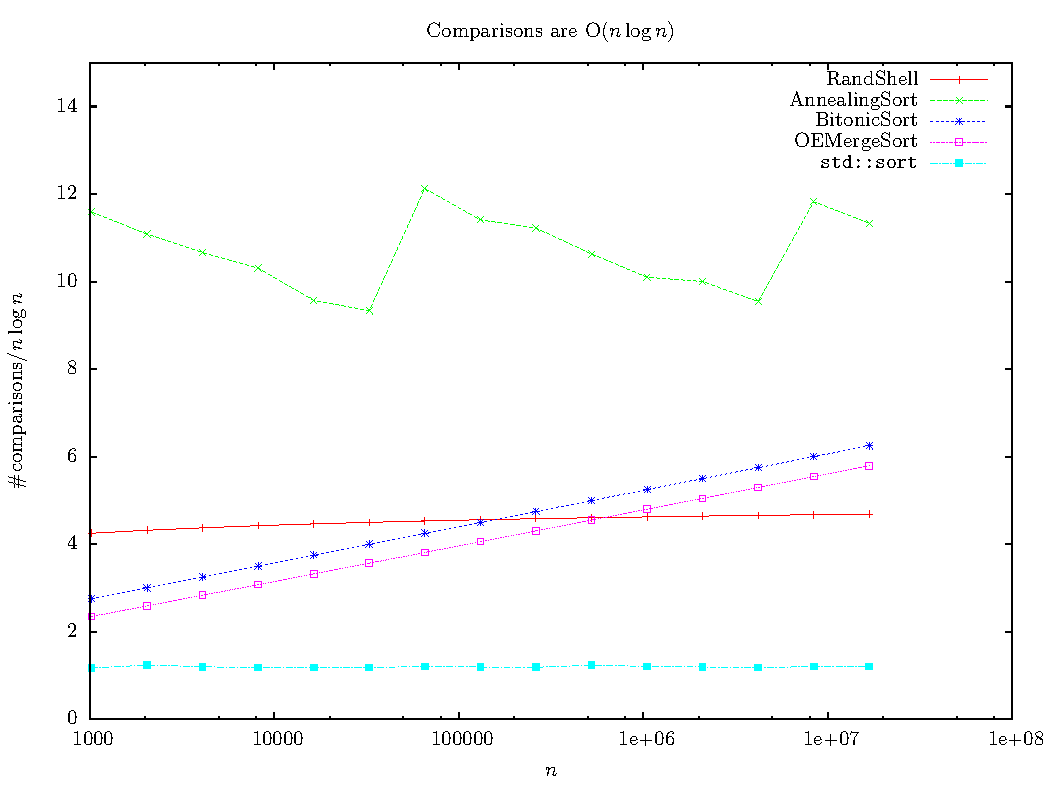
\includegraphics[width=\textwidth]{graphs/Performance/nlogncomparisons.pdf}
\caption{Comparison count of the algorithms}
\label{fig:Performance:comparisons}
\end{figure}


Now, let us look at the running times of the algorithms, which are shown in Figure~\ref{fig:Performance:time}.
Unfortunately, running times are nowhere near as predictable or consistent with theory as the amount of comparisons, but they are however of great practical importance.

Randomized Shellsort appears slow compared to the other algorithms, especially considering its low amount of comparisons compared to the sorting networks, and at input sizes larger than $1 \times 10^6$, it appears to grow faster than $O (n \log n)$. An explanation for the slow running time of Randomized Shellsort is given in Section~\ref{sec:PerformanceInstructions}. At sizes between $1.6 \times 10^4$ and $1 \times 10^6$, we see the expected running time of $O( n \log n)$, which is consistent with theory.

Both Bitonic Sort and Odd-Even Mergesort show good performance, but they are growing in $O ( n \log^2 n)$. We see that Odd-Even Mergesort is slower than Bitonic Sort, despite performing fewer comparisons, which is interesting. Unlike Randomized Shellsort and Annealing Sort, there appears to be no immediate problem of going beyond $1 \times 10^6$ elements for these two algorithms.

Annealing Sort is slow, as expected from the high number of comparisons. At sizes between $1.6 \times 10^4$ and $1 \times 10^6$, the algorithm follows the $O(n \log n)$ expected complexity well, but performance degrades rapidly at the $1 \times 10^6$ element mark. This performance degradation will, like that of Randomized Shellsort, be further discussed in Section~\ref{sec:PerformanceInstructions}.


\begin{figure}
\center
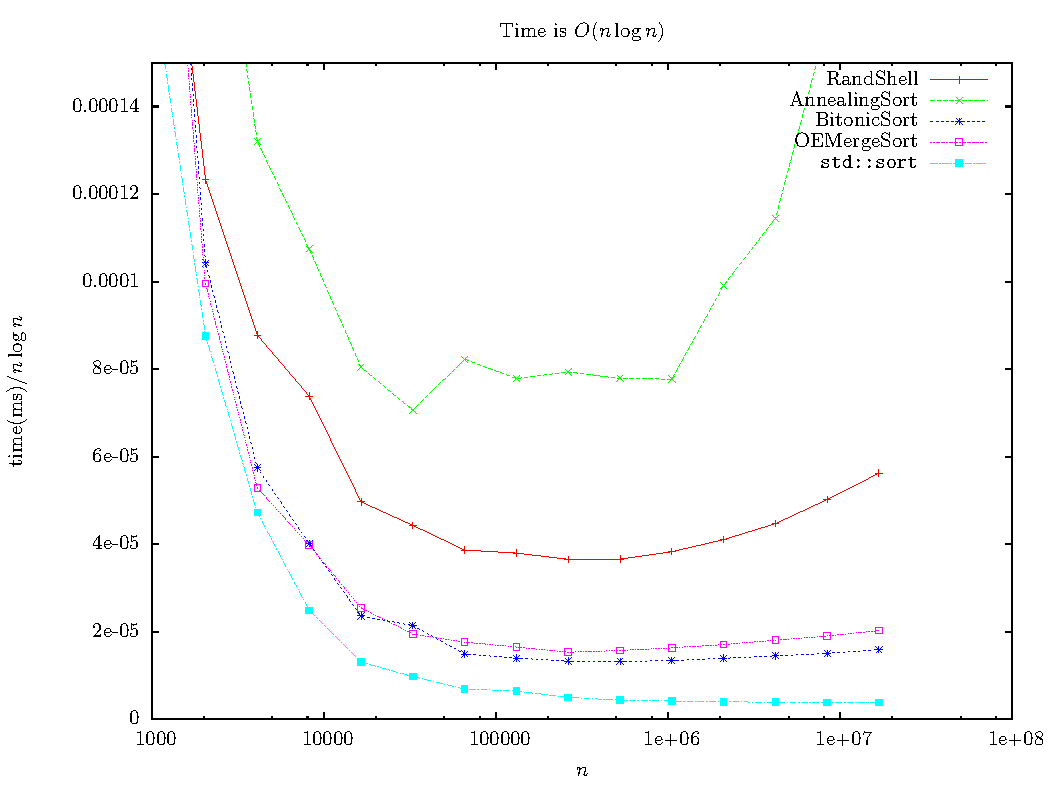
\includegraphics[width=\textwidth]{graphs/Performance/nlogntime.pdf}
\caption{Running time of the algorithms}
\label{fig:Performance:time}
\end{figure}


\subsection{Instructions and Cache Misses}
\label{sec:PerformanceInstructions}

Having shown that the algorithms behave somewhat reasonably, let us move on to show why performance is not directly tied to the number of comparisons, and why some algorithms run into problems at the $1 \times 10^6$ element mark.

First, let us look at the amount instructions performed per comparison, as shown in Figure~\ref{fig:Performance:instructions:comparisons}.
Note that all of algorithms converge towards a constant amount of instructions per comparison, which bodes well for their implementation.

We see that Randomized Shellsort has a high number of instructions per comparison, which helps explain why it is outperformed by the $O (n \log^2 n)$ sorting networks, despite having a similar or lower number of comparisons.

Bitonic Sort performs a low amount of instructions per comparison, which is what makes it outperform Odd-Even Mergesort despite using higher number of comparisons. The high number of instructions performed by the Odd-Even Mergesort can be atributed to the procedure of moving odd and even elements around between buffers.

Annealing Sort actually performs relatively few instructions per comparison, since it is a simple algorithm. This is unfortunately not enough to balance out the high number of comparisons in terms of final running time.

\begin{comment} %IM INVISIBRU
\begin{figure}
\center
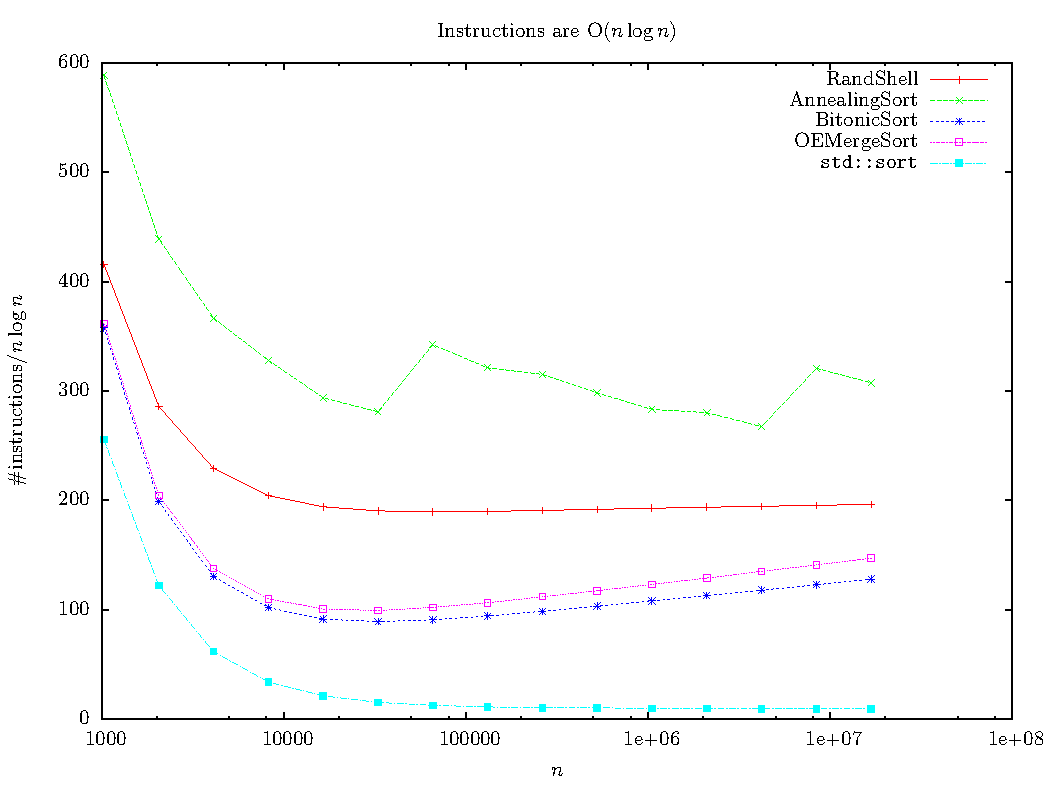
\includegraphics[width=\textwidth]{graphs/Performance/nlogninstructions.pdf}
\caption{Instruction Count of the algorithms}
\label{fig:Performance:instructions:nlogn}
\end{figure}
\end{comment}


\begin{figure}
\center
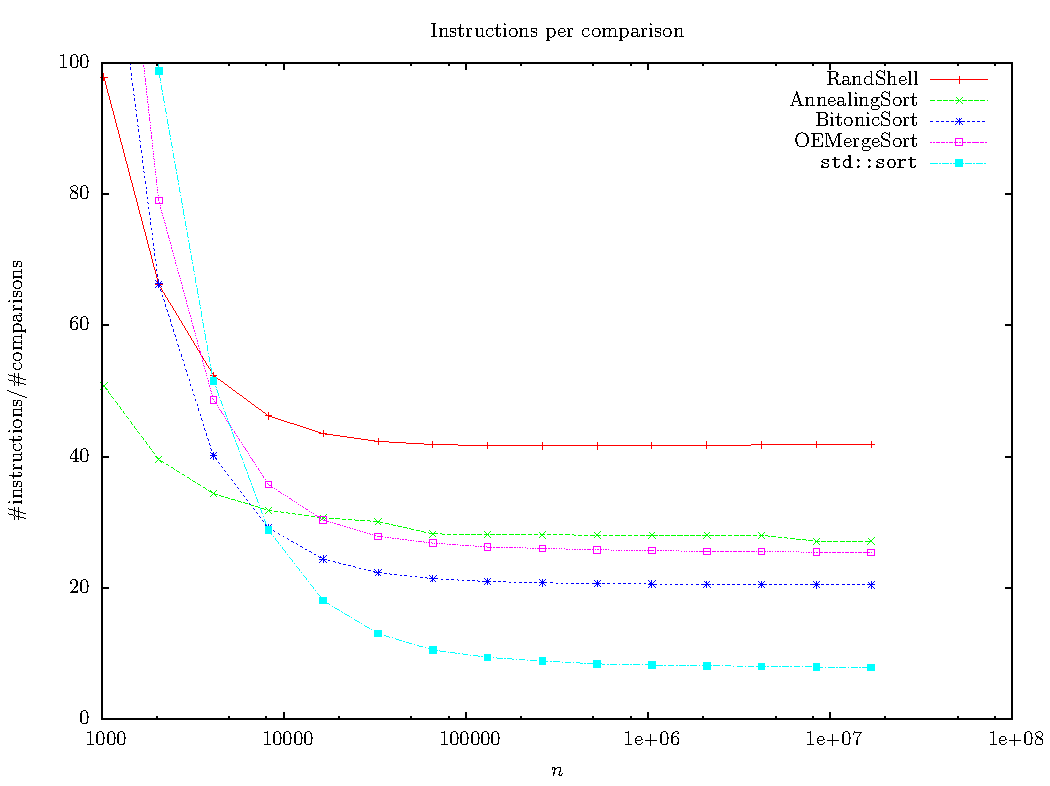
\includegraphics[width=\textwidth]{graphs/Performance/instructionscomparison.pdf}
\caption{Instructions per Comparison of performed by the algorithms}
\label{fig:Performance:instructions:comparisons}
\end{figure}

Now, let us move on to cache misses. Cache misses can be seen in Figure~\ref{fig:Performance:cachemisses}.
Keep in mind that test are performed on a machine with 4MB cache using signed 32-bit integers, which places the amount of elements fitting into cache at about $1 \times 10^6$ elements.

Randomized Shellsort and Annealing Sort both start having major cache problems around the cache limit, which explains their performance problems when going above  $1 \times 10^6$ elements. The high number fo cache misses is a direct effect of their random access patter when comparing data, which both prevents memory preloading, and leads to big jumps in accessed indexed of elements.

Bitonic Sort and Odd-Even Mergesort both perform few cache misses, since they both work locally in terms of data access, and rely on linear access patterns allowing the memory prefetcher to lower latency when crossing a cache line border.

\begin{figure}
\center
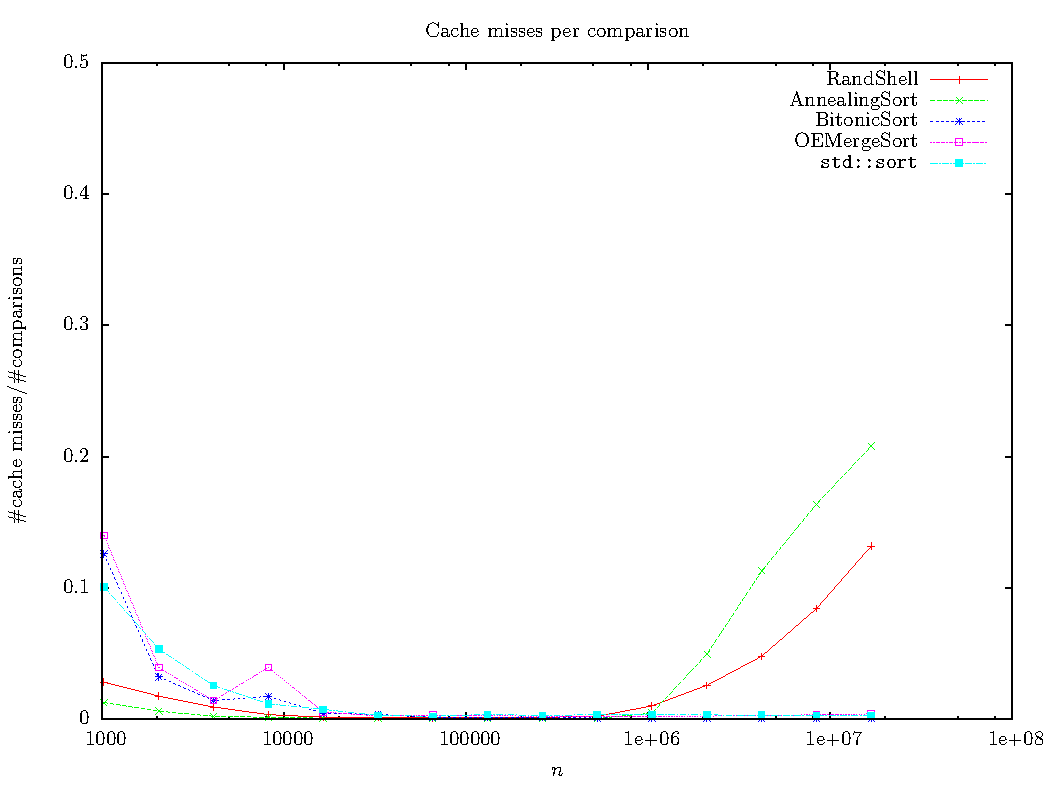
\includegraphics[width=\textwidth]{graphs/Performance/cache-misses.pdf}
\caption{Cache Misses of the algorithms}
\label{fig:Performance:cachemisses}
\end{figure}

\subsection{Branch Mispredictions}

Throughout this section, we have made many interesting observations about the data-oblivious algorithms, but unfortunately, they seem to be outperformed by \texttt{std::sort} on every single performance metric. Though there is still one point in which they can outperform classic data-dependent sorting algorithms.

Figure~\ref{fig:Performance:branchmisses} shows the number of branch mispredictions performed by the different algorithms.

The data-oblivious algorithms can all be seen to perform a number of branch mispredictions that is either almost negligible, or $O (n)$, since the \texttt{Compare-Exchange} operation can be done without branching. \texttt{std::sort}, on the other hand, performs a number of branch mispredictions that is $O(n \log n)$, since it is must perform a branch for each comparison, and assuming uniformly random input data, it will not be possible to reliably predict the result of this branch. 

\begin{figure}
\center
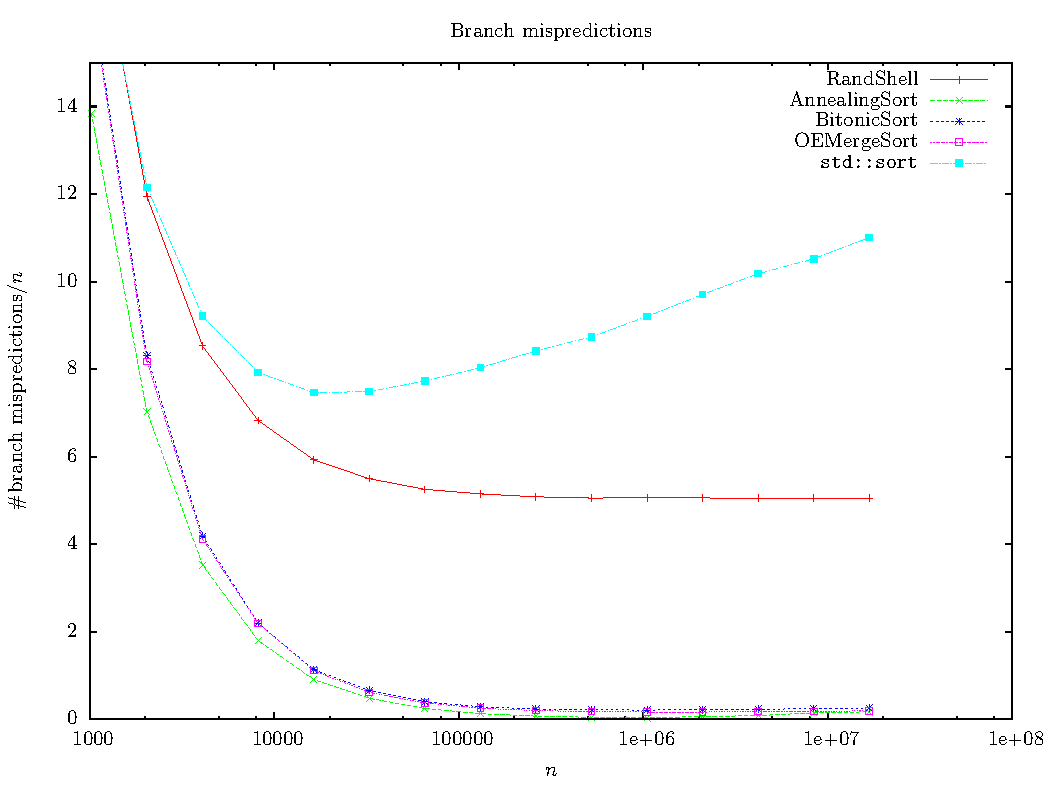
\includegraphics[width=\textwidth]{graphs/Performance/branch-misses.pdf}
\caption{Branch Mispredictions of the different algorithms}
\label{fig:Performance:branchmisses}
\end{figure}

\subsection{Experiment Results}

The experiment shows that both of the new algorithms perform according to their expected running times of $\Theta(n \log n)$, for a significant part of the experiment. These newer algorithms are however hindered by a large instruction overhead and a poor cache performance, and are therefore somewhat slow in practice.

Randomized Shellsort is notable in that it performs a low number of comparisons compared to Bitonic Sort and Odd-Even Mergesort as $n$ increases, which might prove useful in the field of secure multi-party computations.

Annealing Sort seems entirely unsuited for practical use.

